% LATEX TEMPLATE 
% adapted from https://infinitedescent.xyz/latex/ by wade_

\documentclass[11pt]{article}

% Edit the following to change the title, author name and date
\title{Calc in 3d Notes}
\author{saffron\_}
\date{}

% Packages
\usepackage{amsmath}
\usepackage{amsfonts}
\usepackage{amssymb}
\usepackage{amsthm}
\usepackage{enumerate}
\usepackage{geometry}
\usepackage{graphicx}
\usepackage{hyperref}
\usepackage{multicol}
% \usepackage[colorlinks=true,linkcolor=magenta]{hyperref}

% Page setup
\setlength{\parskip}{10pt}
\setlength{\parindent}{0pt}
\geometry{
    paper={letterpaper}, % Change to 'a4paper' for A4 size
    marginratio={1:1},
    margin={1in}
}

% Theorem environments
\theoremstyle{definition}
\newtheorem{theorem}{Theorem}
\newtheorem{lemma}[theorem]{Lemma}
\newtheorem{corollary}[theorem]{Corollary}
\newtheorem{proposition}[theorem]{Proposition}
\newtheorem{definition}[theorem]{Definition}
\newtheorem{example}[theorem]{Example}

% Custom per each document
\newcommand{\addsection}[1]{\newpage\section*{#1}\addcontentsline{toc}{section}{#1}} % for adding \section*{} sections to \tableofcontents
\newcommand{\bb}[1]{\mathbb{#1}} % love of my life
% \newcommand{\floor}[1]{\left\lfloor #1 \right\rfloor}
% \newcommand{\ceil}[1]{\left\lceil #1 \right\rceil}

\graphicspath{ {./media/} }

\begin{document}
\maketitle
\tableofcontents

%%%%%%%%%%%%%%%%%%%%%%%%%%%%
%% Start of document body %%
%%%%%%%%%%%%%%%%%%%%%%%%%%%%

\addsection{test}
Hello world! Did you know that $3^2 + 4^2 = 5^2$?
\begin{multicols}{3}
  [
  All human things are subject to decay. And when fate summons, Monarchs must obey.
  ]
  

Lorem ipsum dolor sit amet, consectetur adipiscing elit. Ut finibus eros et nisi porttitor, ultrices tempor diam blandit. Praesent bibendum nibh sed volutpat facilisis. Vestibulum massa ex, congue nec felis quis, maximus ultricies erat. Mauris lobortis nibh ut tempus placerat. Proin ut condimentum nibh. Proin bibendum ligula nibh, at pulvinar nisl efficitur eu. Fusce venenatis, purus ut lacinia malesuada, nisi turpis sollicitudin enim, sed tristique elit ex a mi. Fusce laoreet sodales purus at blandit. Interdum et malesuada fames ac ante ipsudm primis in faucibus.  \end{multicols}
  
\newpage
\addsection{Appendix}
\subsection*{matrices, 3x3 determinants}
Recall that a elements of a matrix are enumerated $a_{ij}$ where $i$ is column and $j$ is row, both 1-indexed. 
\[\begin{bmatrix}
  a_{11} & a_{12} & a_{13}\\
  a_{21} & a_{22} & a_{23}
\end{bmatrix}\]
\begin{figure}[h]
  \centering
  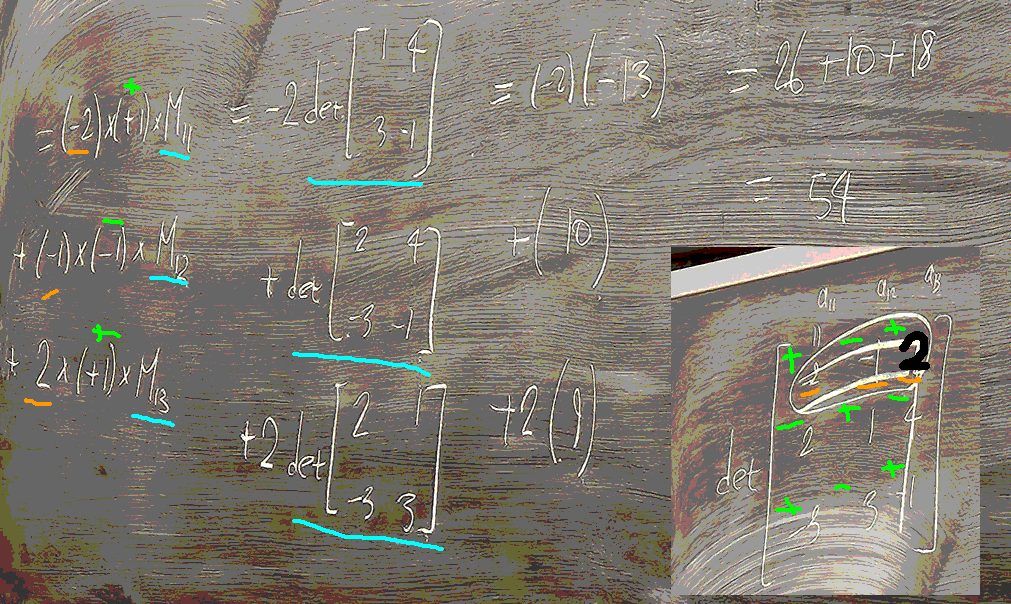
\includegraphics[scale=0.5]{3x3determinant}
\end{figure}

Recall that the minor of the matrix element here is the 2 by 2 determinant when you take away the row and column of the element in a 3 by 3 matrix.  Picking an arbitrary row (or even column), with $a_{ij}$ being an element and $M_{ij}$ being a minor, a 3 by 3 determinant is calculated by 
\[ \sum_{j=1}^{3} (-1)^{i+j} a_{ij} M_{ij} \]
In the figure above, $(-1)^{i+j}$ is in green, $a_{ij}$ in orange, and $M_{ij}$ in blue.


%%%%%%%%%%%%%%%%%%%%%%%%%%%%
%% End of document body   %%
%%%%%%%%%%%%%%%%%%%%%%%%%%%%
\end{document}
